\section{Zusammenfassung}



\begin{itemize}
    \item \textbf{Anforderungen} sind Bedürfnisse der Stakeholder und Kunden an das Softwaresystem.
    \item Vor der Erarbeitung der Anforderung sollte sich über eine \textbf{Domänenanalyse} mit den Begriffen und Konzepten der Domäne vertraut gemacht werden.
    \item daraufhin wird der wirtschaftliche Nutzen, den sich der Kunde verspricht, als \textbf{Geschäftsanforderungen} in einem \textbf{Lastenheft} festgehalten.
    \item Anschließend werden die Anforderungen aller involvierten Personen (\textbf{Stakeholder}) ermittelt, insbesondere der \textbf{Endanwender}.
    \item Diese Anforderungen werden grob unterteilt in \textbf{funktionale} und \textbf{nicht-funktionale} Anforderungen.
    \item funktionale Anforderungen sind hierbei die Funktionen, der der Endanwender von dem System erwartet.
        \begin{itemize}
            \item funktionale Anforderungen werden als \textbf{Use Case} oder \textbf{User Story} erfaßt.
            \item Anwendungsfälle (Use Cases) können hierbei sehr detailliert und formell beschrieben werden.
            \item User Storys sind i.d.R. wenig detailliert und beschreiben nur kurz den Umgang des Endanwenders mit dem System.
            \item Steueranwendungen (Hardware) können auch \textbf{Ereignistabellen} verwendet werden.
        \end{itemize}
    \item nicht-funktionale Anforderungen sind technische und organisatorische Anforderungen, die üblicherweise in Form von Listen gesammelt werden
    \item \textbf{Regeln}, und \textbf{Formate von Daten} werden gesondert erfaßt, als \textbf{Business Rules} in Listen bzw. in \textbf{Datadictionaries} und der Angabe von \textbf{Mengengerüste}.
    \item Die Aufstellung all dieser Anforderung wird bei dem \textbf{Wasserfallmodell} oft in Form des \textbf{Pflichtenhefts} realisiert.
\end{itemize}


\begin{figure}
    \centering
    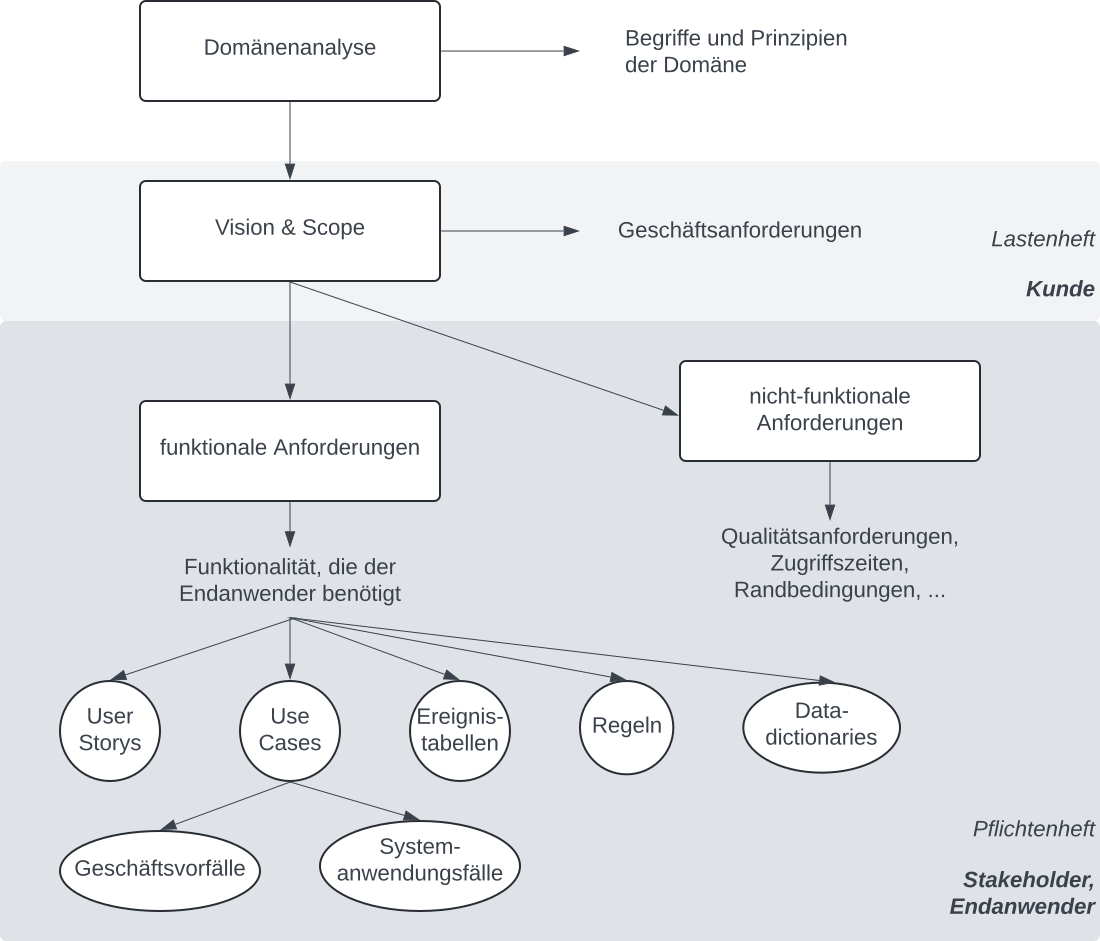
\includegraphics[scale=0.35]{chapters/Requirements Engineering/img/anforderung}
    \caption{Abfolge der Erfassung verschiedener Anforderungen. (Quelle: eigene)}
    \label{fig:anforderung}
\end{figure}